\documentclass{article}
\usepackage[utf8]{inputenc}
\usepackage[margin=1in]{geometry}
\usepackage{graphicx}

\usepackage{setspace}
\doublespacing

\usepackage{hyperref}
\hypersetup{
    colorlinks=true,
    linkcolor=blue,
    filecolor=magenta,      
    urlcolor=cyan,
    pdftitle={Overleaf Example},
    pdfpagemode=FullScreen,
    }

\urlstyle{same}

\begin{document}


\section{Analysis Motivation}
An alcohol company that owns a chain of stores across Russia recently had ran a successful wine promotional in Saint Petersburg. Due to a limited budget, the company will not be able to run a promotion in all regions. Hence, the marketing team has tasked me to identify ten other regions to run a successful wine promotion. To do this, we will implement a clustering model that will return regions with similar purchasing habits as St Petersburg. These regions will then be analysed further based on their recent wine sales to pinpoint the best ten regions for a future wine promotion.

\section{Exploratory Data Analysis}
The dataset used in this project can be found at the DataCamp \href{https://github.com/datacamp/careerhub-data}{careerhub-data} repository. Specifically, we will be focusing on the ``Alcohol Consumption in Russia'' dataset. This dataset consists of the following seven columns. 

\begin{table}[!htb]
    \centering
    \begin{tabular}{c|ccc}\hline
        Description & Type & Non-Null Count & Data Type\\ \hline
         Year &  numerical & 1615 & int64 \\
         Region & categorical & 1615 & object \\
         Wine & numerical& 1552  & float64\\
         Beer & numerical & 1557 & float64\\
         Vodka & numerical& 1554 & float64\\
         Champagne & numerical& 1552 & float64\\
         Brandy & numerical& 1549 & float64\\\hline
    \end{tabular}
    \caption{Type and Missing Data}
    \label{tab:data_type}
\end{table}


\noindent In the reaming parts of this section we will go through the motions of exploring data. This will give us a deeper understanding of the data and help uncover any issues within it. So let us get started. Firstly, the shape of the data is $(1615 \times 7)$, and thus very small, as opposed to most data sets. Secondly, we will run some basic statistics on the numerical data using the describe method from pandas.

\begin{table}[!htb]
    \centering
    \begin{tabular}{c|c|c|c|c|c}
    \hline
        & year & wine & beer& vodka & champagne\\\hline
        count & $1615.000000$ & $1552.000000$ & $1557.000000$ & $1554.000000$ & $1552.000000$ \\
        mean & $2007.000000$  & $5.628144$ & $51.206148$ & $11.818694$ & $1.313177$ \\
        std  & $5.478922$ & $2.813208$ & $25.372821$ & $5.128806$ & $0.797956$\\
        min  &  $1998.000000$ & $0.100000$ & $0.400000$ & $0.050000$ & $0.100000$\\
        $25\%$& $2002.00000$ & $3.575000$ & $32.400000$ & $8.300000$ & $0.800000$\\
        $50\%$& $2007.000000$ & $5.400000$ & $49.970000$ & $11.500000$ & $1.200000$\\
        $75\%$& $2012.000000$ & $7.377500$ & $67.400000$ & $15.000000$ & $1.665000$\\
        max  & $2016.000000$ & $18.100000$ & $207.300000$ & $40.600000$ & $5.560000$\\
        \hline
    \end{tabular}
    \caption{Initial Statistics with Describe}
    \label{tab:inital_stats}
\end{table}


\noindent From Table \ref{tab:data_type}, we can already see that there is some missing data that will need to be dealt with. In fact, the only complete columns are year and region. Before treating the missing data, let's visualize the data using histograms as shown in Figure \ref{fig:Histograms}. It appears that the data is mostly right skewed. Where champagne and brandy have longer tails. On the other hand wine, beer and vodka are closer to normal. 

\begin{figure}[!htb]
    \centering
    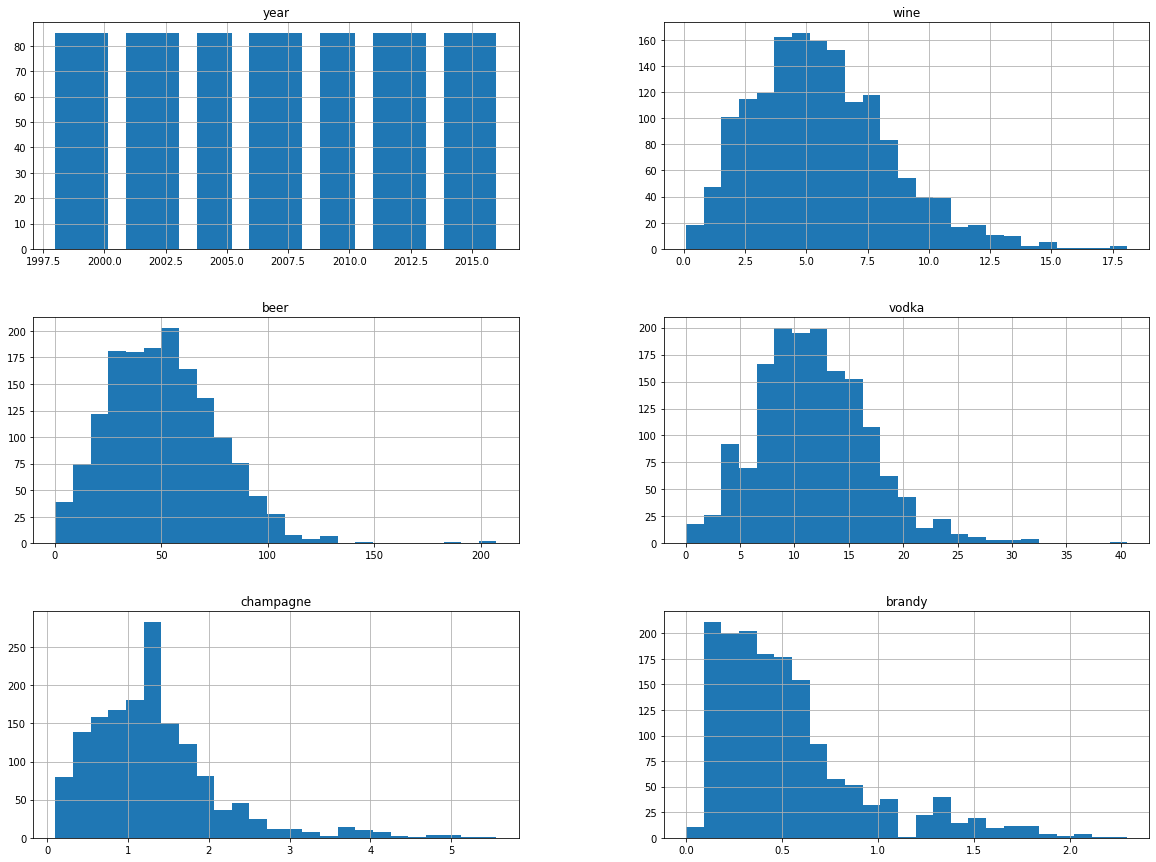
\includegraphics[scale = .42]{output_4_1.png}
    \caption{Histograms}
    \label{fig:Histograms}
\end{figure}

\section{Treating Missing Data} Now we will handle the missing data using one of my personal favorite modules in python, missingo. Using this module we can visualize the distribution of missing data. Note in the following figures, the white ``chuncks'' refer to missing data. In Figure \ref{fig:miss_data}, the missing data is scattered throughout the entire data set. Whereas, in Figure \ref{fig:miss_data_region} the data is arranged by region, and it is clear the missing data occurs in four different regions. After some further analysis the regions of interests are: Chechen Republic, Republic of Crimea, Sevastopol and Republic of Ingushetia.

%====================================================================================
\begin{figure}
    \centering
    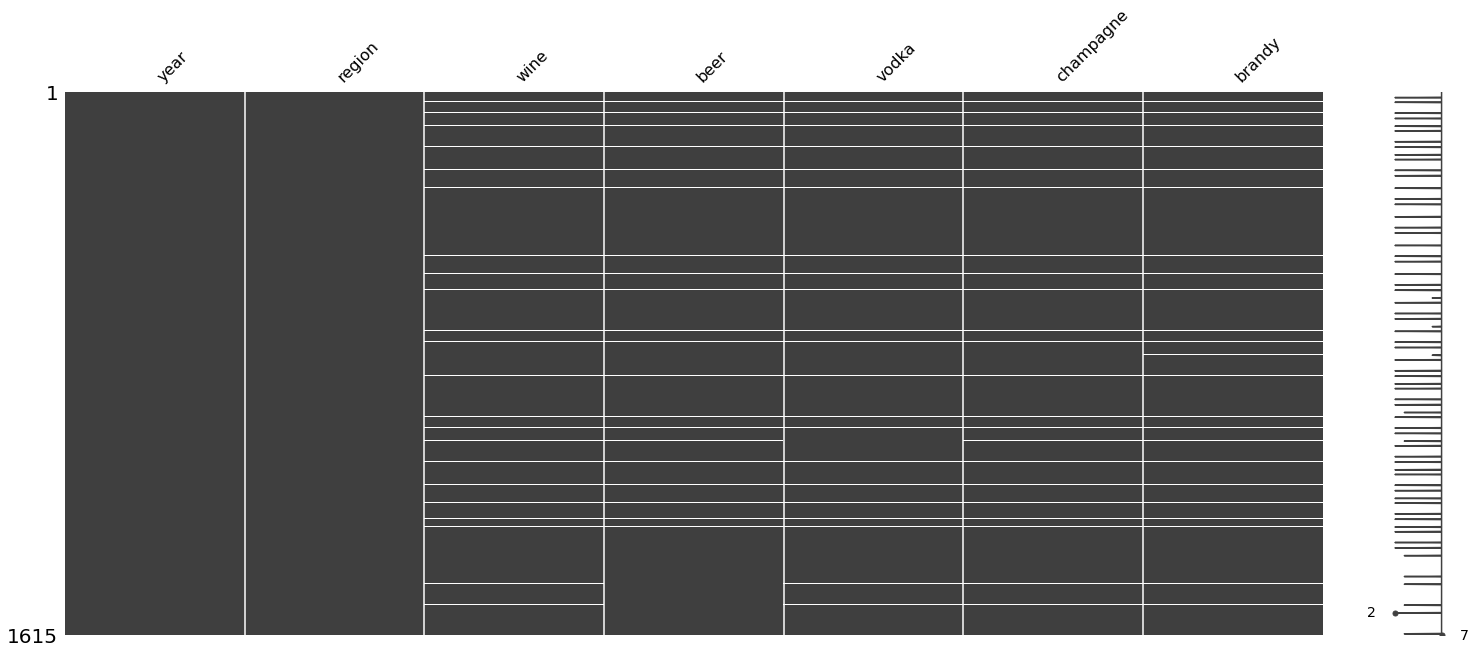
\includegraphics[scale = .3]{Missingo/output_7_1.png}
    \caption{Location of Missing Data}
    \label{fig:miss_data}
\end{figure}

\begin{figure}[!htb]
    \centering
    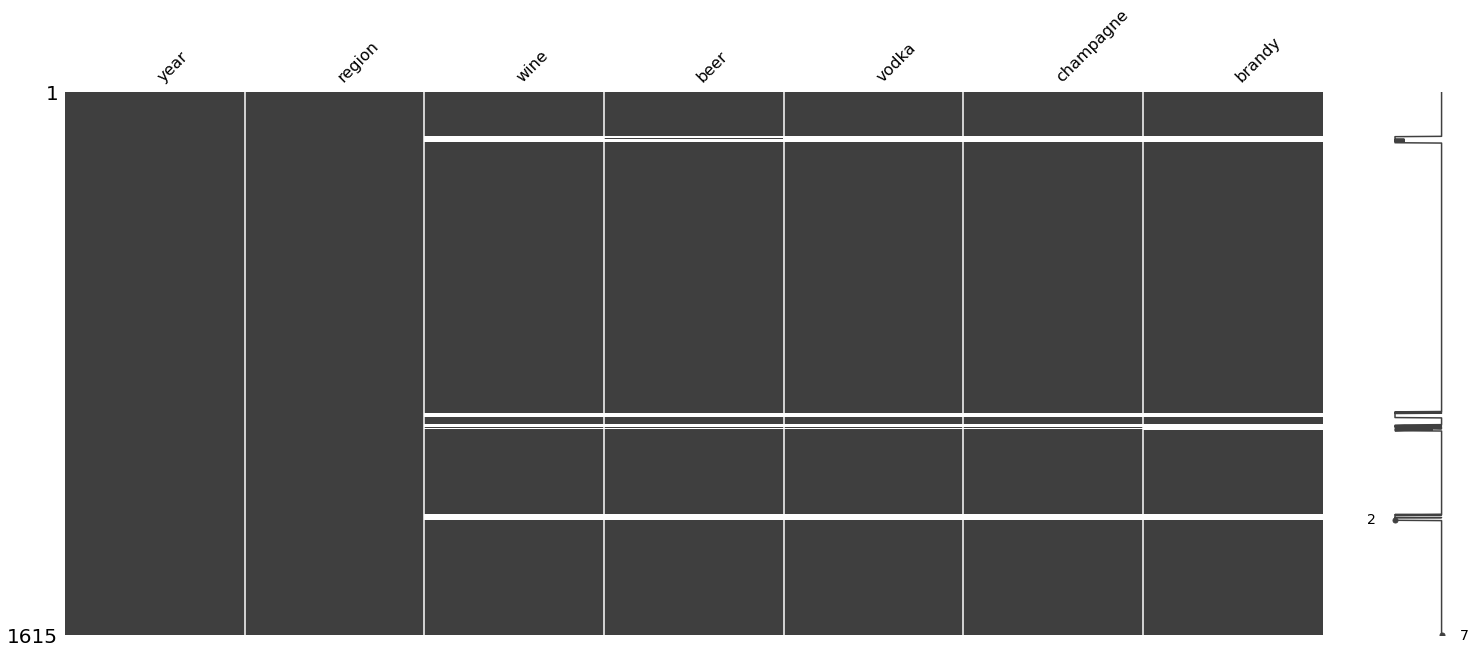
\includegraphics[scale = .3]{Missingo/output_8_1.png}
    \caption{Location of Missing Data Grouped by Region}
    \label{fig:miss_data_region}
\end{figure}
\newpage

\noindent In order to handle the missing data, any fully incomplete rows will be dropped. We can retain other rows of missing data by imputing the mean of its corresponding region. With this in place, we now have a complete data set. However, we must treat outliers. It is standard practice to treat outliers but more importantly they can pose a massive threat in terms of the quality of our future clustering model.

\section{Treating Outliers}
Treating outliers can be tricky. We will first use box plots to visualize any data which reaches far beyond the mean. These points will be the main suspects for the outliers. Secondly we will evaluate the z-scores as a double checking method. Lastly we will pinpoint where the outliers are located within the data and deal with them accordingly.

\begin{figure}[!htb]
    \centering
    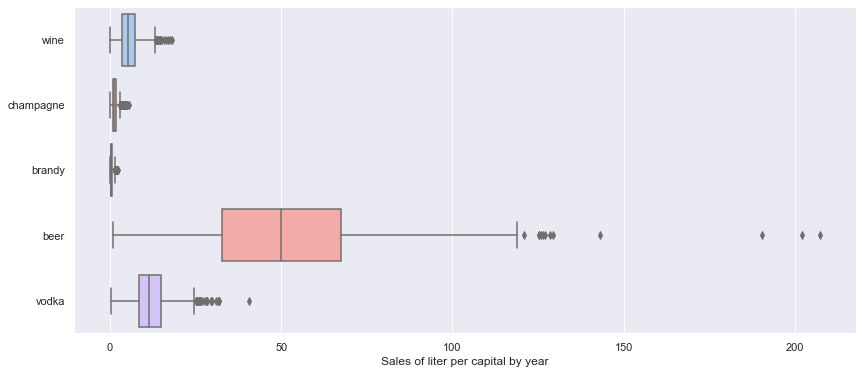
\includegraphics[scale = .4]{BoxploTs/output_18_1.png}
    \caption{Box plot of each alcohol type}
    \label{fig:box_plot_1}
\end{figure}
\noindent Immediately, from Figure \ref{fig:box_plot_1} the top three data points for beer and the top data point for vodka are suspected outliers. Since the other three alcohol types are difficult to interpret due to scaling. We will create a separate plot for these categories.\newline

\begin{figure}[!htb]
    \centering
    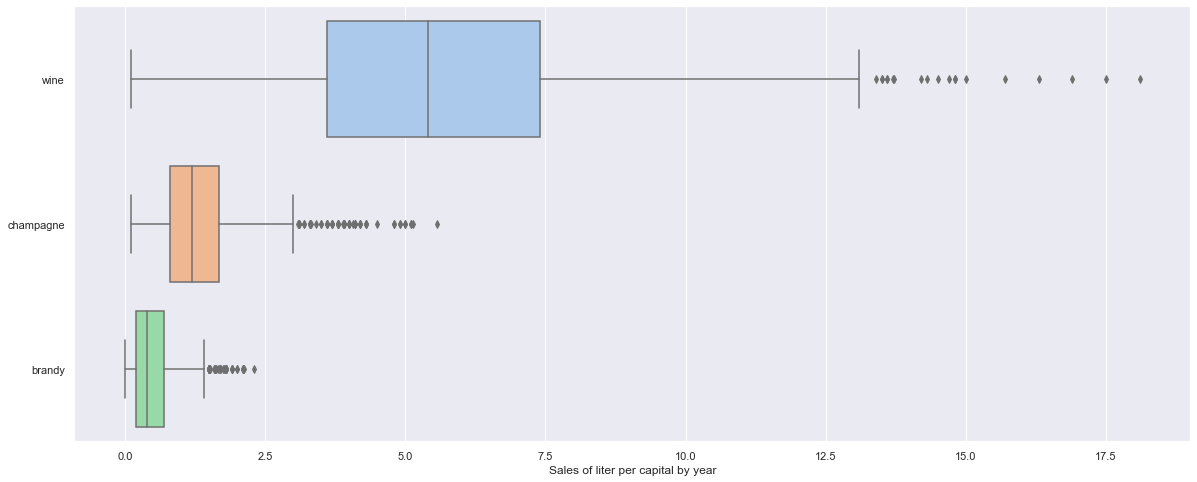
\includegraphics[scale = .3]{BoxploTs/output_19_1.png}
    \caption{Box plot of wine, champagne, and brandy}
    \label{fig:box_plot_2}
\end{figure}
\noindent From Figure \ref{fig:box_plot_2} the suspected outliers are the top five data points for wine, top five data points for champagne, and the top data point for brandy. Next we shall check the z-scores for the top 5 data points. Recall the z-score of a data point signifies how many standard deviations away from the mean the data point is. The z-score can be positive or negative number, indicating the data point is above or below the mean respectively.

\begin{table}[!htb]
    \centering
    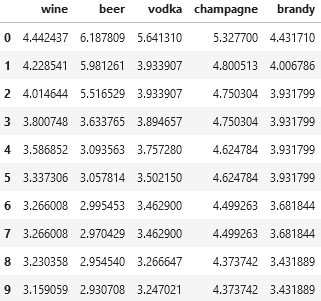
\includegraphics[scale = .7]{Graphs/zscore.png}
    \caption{Top 10 z-scores (descending)}
    \label{tab:zscore}
\end{table}

\noindent Comparing the list of suspected outliers to Table \ref{tab:zscore}, our suspicions can be put to rest. The data points discussed in the prior paragraph are far beyond the mean, and should be imputed in some way. Each of the data points mentioned will be filled with the mean alcohol sales during the year where the outlier occurred. 

\section{K-Means Clustering}
Now that the data has been processed we can work toward picking our model. As the section title suggests we will be utilizing the K-means clustering algorithm. This is an unsupervised machine learning algorithm which aims at clustering regions into similar groups. In this case, ``similar'' refers to regions which share analogous historical wine sales. Since we know that St Petersburg had a successful wine promotion, we can check its cluster for other potential regions for a future wine promotion. However, we have a limited budget, so we may need to dig deeper beyond just selecting ten random regions in St Petersburg's cluster. 

\subsection{Prepping the Data}
In order to use the K-Means algorithm we need to have data with low variance, and similar means. A quick fix for this is to normalize our wine sales data. That is to do the following:
\begin{enumerate}
    \item Create a pivot table with regions as the row headers and years as the column headers
    \item Fill the pivot table with wine sales
    \item Divide each year column by the max wine sale for that year.
\end{enumerate}

\noindent By doing so, all the wine sales data is within the range [0,1], and is now fitted for the K-Means algorithm. Moreover, normalized data is great for heat maps. In Figure \ref{fig:heatmap_r} we can see the overall trend of wine sales for each region. Notice, the darker the cell, the closer to the max it is.

\begin{figure}[!htb]
    \centering
    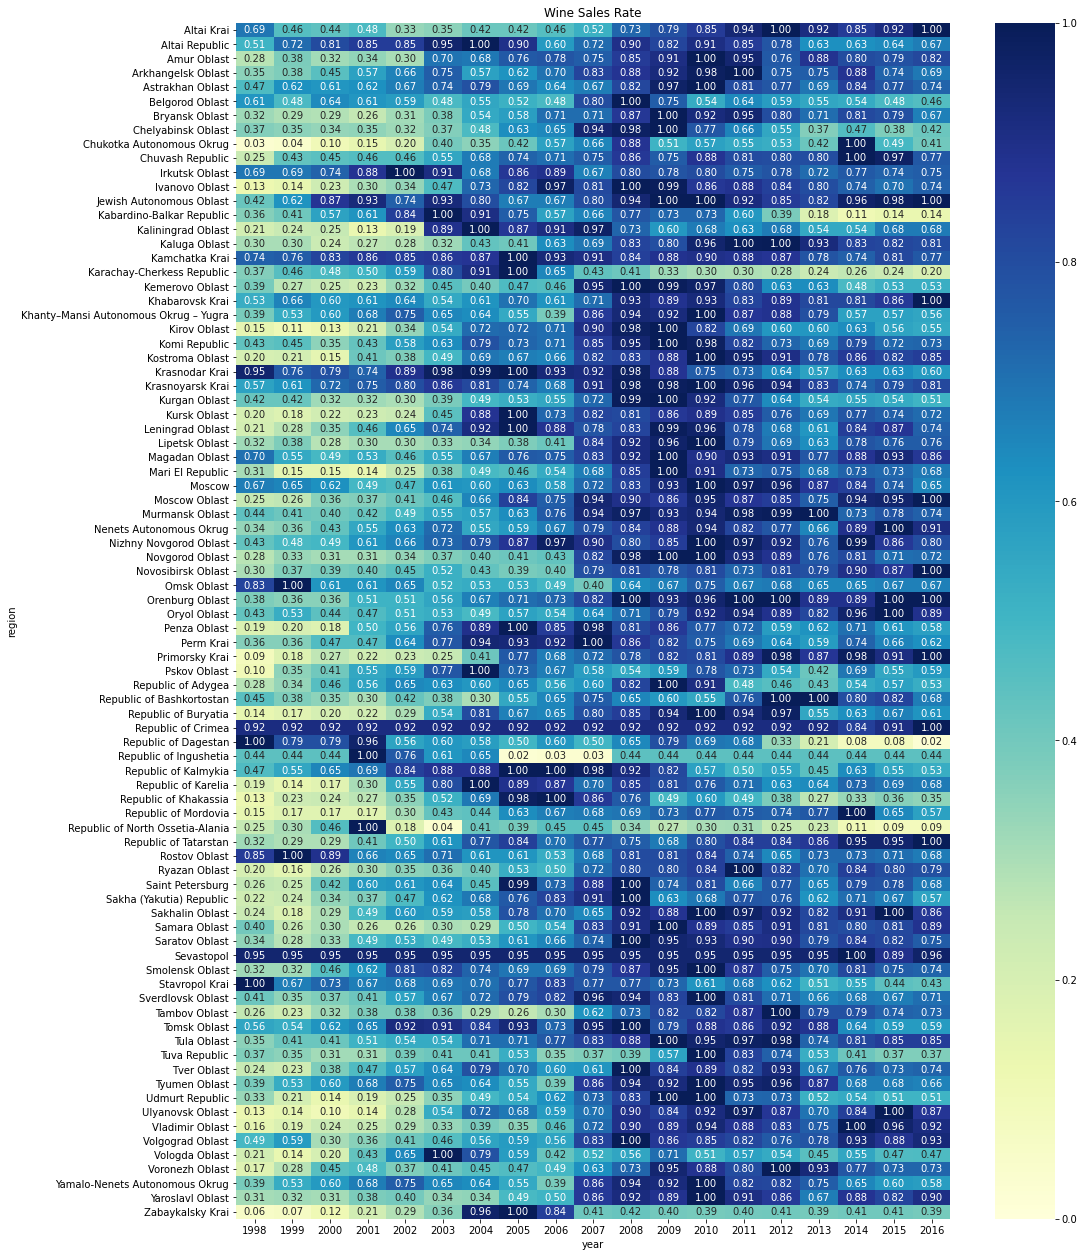
\includegraphics[scale = .42]{Graphs/heatmap_region.png}
    \caption{Heat Map of Regional Wine Sales}
    \label{fig:heatmap_r}
\end{figure}

\subsection{Elbow Method}
A major drawback to the K-Means algorithm is having to specify the number of clusters, $k$. The elbow method will help remedy this issue. Essentially, the elbow method works by running the K-Means algorithm $n$ number of times. Then comparing the mean inertia at each iteration of $n$. Inertia in this context refers to the distance from each instance (data point) to its closest cluster. Note as the number of clusters approach the number of instances, the inertia tends to 0. Thus, it does not suffice to take the higher number of clusters to minimize inertia. Rather you want to pick the number of clusters, $k$ around the point where you have inertia but $k+1$ does not lower inertia by a substantial amount. In this project, we will select $n = 29$. Therefore, the K-Means algorithm was ran $29$ times, keeping track of the mean inertia at each iteration. In Figure \ref{fig:elbow} we can see the graph of the number of clusters $k$ versus the mean inertia. Since the drop-off of inertia is minuscule from $k=4$ to $k=5$, we will take $k=4$ to be the number of clusters for this analysis.

\begin{figure}[!htb]
    \centering
    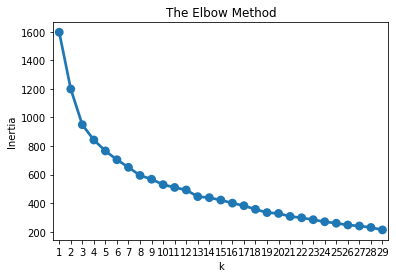
\includegraphics[scale = .7]{Graphs/elbow_method.png}
    \caption{Line Plot: Number of Clusters versus Mean Inertia}
    \label{fig:elbow}
\end{figure}
%By checking the cluster which contains St Petersburg, we will be able to find other regions where a wine promotion may be beneficial to run.  

\subsection{Post K-Means Analysis}
Now that we have the four clusters, we should check which regions are in the same cluster as St Petersburg. Again, we are interested in this cluster since the wine promotion was success full in St Petersburg, and we want to recreate this success. In Figure \ref{fig:heatmap_c} we can see the overall trend of wine sales for regions in each cluster. For example, cluster $0$ has a progressive increase in wine sales, peaking around 2008, with fluctuations after 2008. It turns out that St Petersburg is apart of cluster 0, so this cluster will be important. In fact, we could end our analysis here by randomly taking ten regions from this cluster and running the wine promotion there. Recall however, our budget is small, so let's get more detailed.\newline

\begin{figure}[!htb]
    \centering
    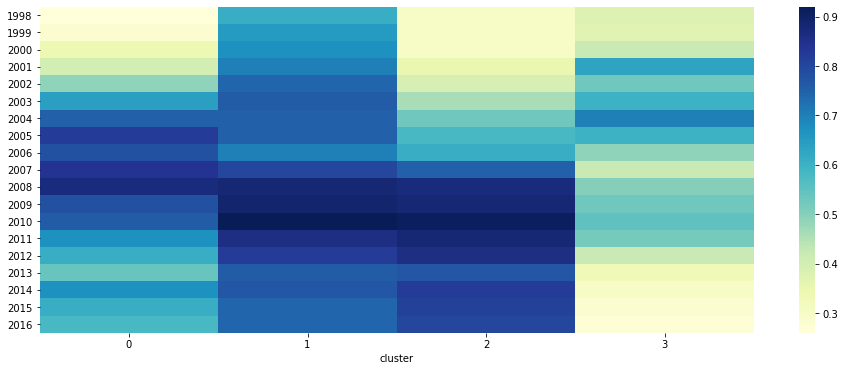
\includegraphics[scale = .5]{Graphs/heatmap_cluster.png}
    \caption{Heat Map of Wine Sales Trend per Cluster}
    \label{fig:heatmap_c}
\end{figure}

\noindent In figure \ref{fig:Cluster 0 Linear Regression} we can see the different regression lines for each region. Of course the regions with promising, positive slopes will be of most interest. However, we need some way of ranking regions to pick the top ten regions most likely to have a successful wine campaign. By scoring regions based on the slope of their regression line, and average wine sales over the recent (four) years, we can arrive at the following ten regions: Republic of Karelia, Kirov Oblast, Leningrad Oblast, Sverdlovsk Oblast, Chukotka Autonomous Okrug, Kaliningrad Oblast, Pskov Oblast, St Petersburg, Kursk Oblast and Penza Oblast. 


\begin{figure}[!htb]
    \centering
    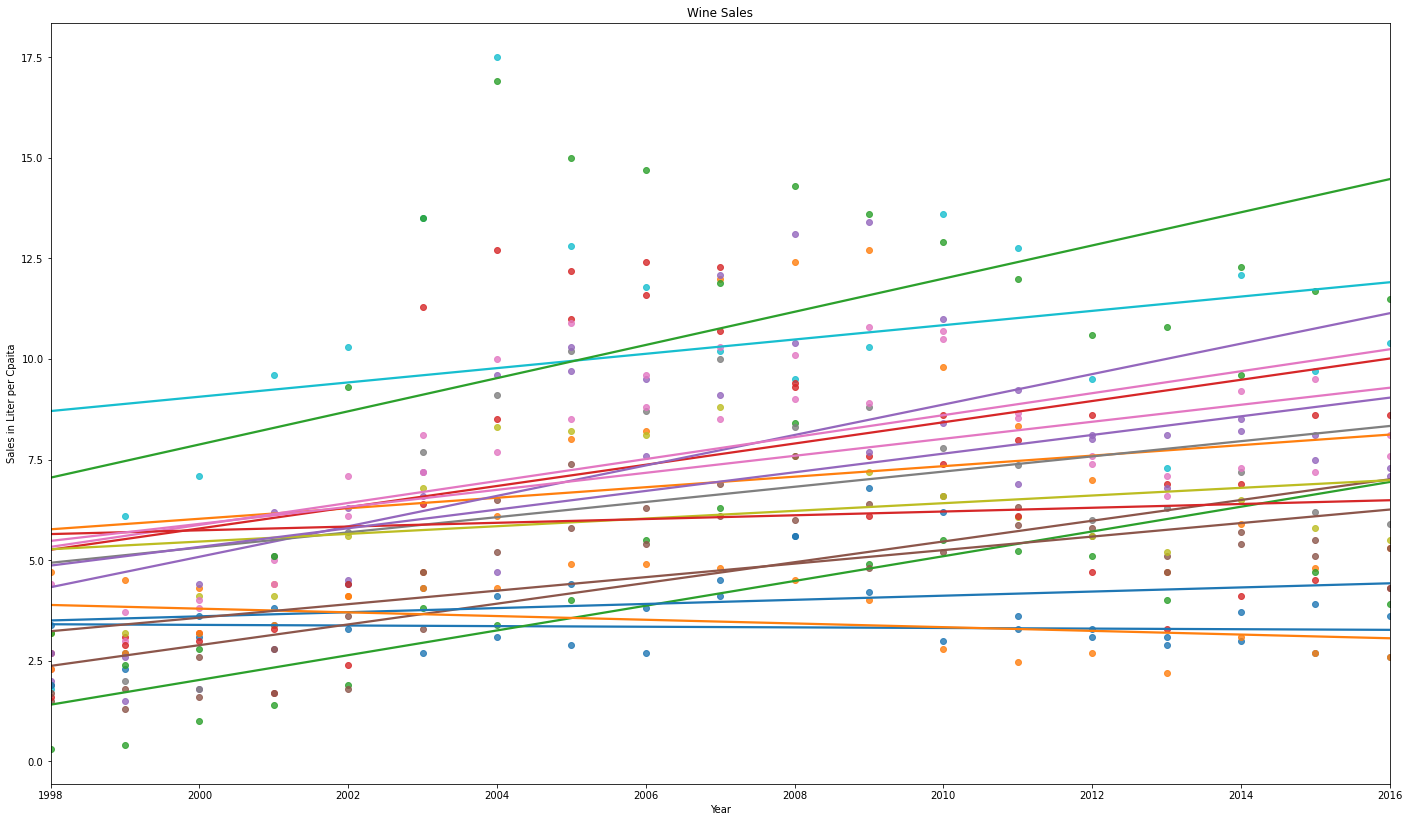
\includegraphics[scale = .3]{Graphs/linear regression.png}
    \caption{Linear Regression of regions in St Petersburg's Cluster}
    \label{fig:Cluster 0 Linear Regression}
\end{figure}

\section{Hierarchical Clustering}

Out of curiosity, a hierarchical clustering algorithm was run on the recent wine sales to see if it would produce a similar result as the K-Means clustering algorithm that was presented earlier. The Hierarchical Clustering produced the deprogram as seen in Figure \ref{fig:dendrogram}.


\begin{figure}[!htb]
    \centering
    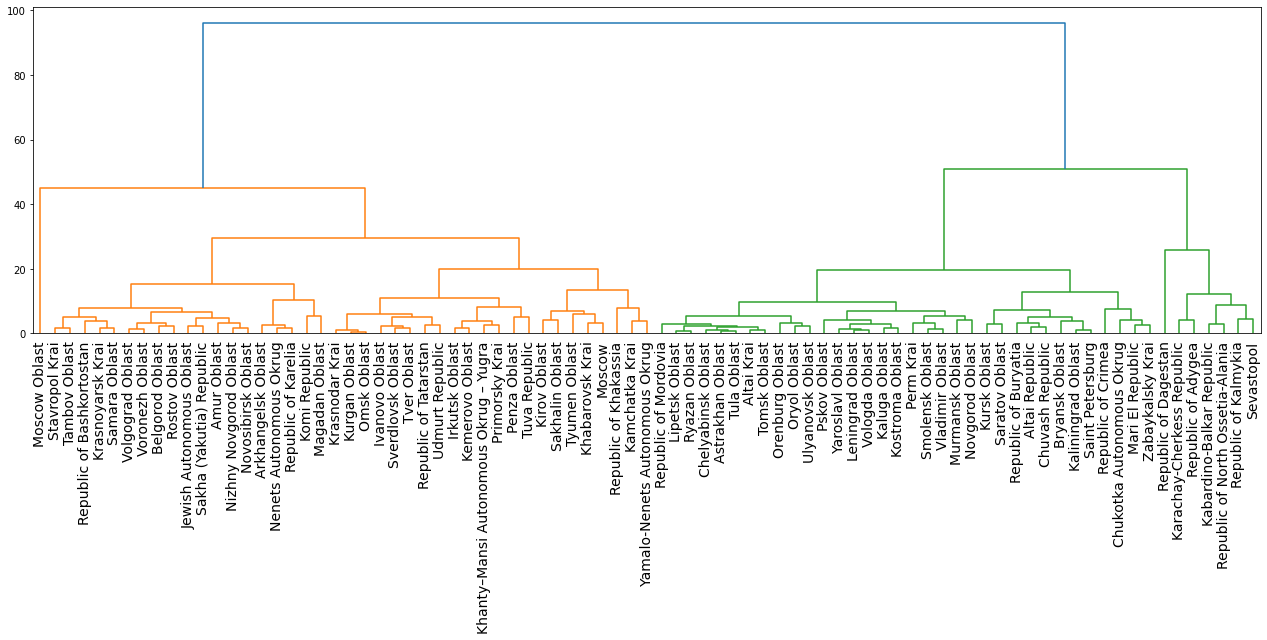
\includegraphics[scale = .35]{Graphs/dendrogram.png}
    \caption{Dendrogram}
    \label{fig:dendrogram}
\end{figure}

\noindent From here we can chose the number of clusters. Selecting four to be the number of clusters, led to St Petersburg being in a cluster of 37 other regions. All top regions picked from the K-Means cluster appeared in the Hierarchical cluster, and thus no new information was gained. However, changing the cluster count to 8, we get a more refined St Petersburg cluster of size seven. In the end there were four regions which were in both the K-Means cluster and the Hierarchical cluster. These four regions are: Chukotla Autonomous Okrug, Kaliningrad Oblast, Kursk Oblast and (unsurprisingly) St Petersburg.

\section{Conclusion}
In the end we have ten regions of interest: Republic of Karelia, Kirov Oblast, Leningrad Oblast, Sverdlovsk Oblast, \textbf{Chukotka Autonomous Okrug},\textbf{ Kaliningrad Oblast}, Pskov Oblast, \textbf{St Petersburg}, \textbf{Kursk Oblast} and Penza Oblast. Note the boldface regions matched with the Hierarchical clustering and K-Means clustering. Hence, we emphasize those as the highest priority regions. Lastly, it is important to mention any aspect of the report which could be improved. First, when faced with missing data or outliers the solution involved imputing reasonable means. However, this is not always the best solution, and other patching methods may prove more adequate. Secondly, transforming the wine data so that it more accurately represents a normal distribution could lead to more precise clustering. Finally we could improve the K-Means clustering by testing different values of $k$ and running the model on new data to check its accuracy. We conclude this report with two final graphs. In the following two figures we are plotting the slope of the linear regression versus the average wine sales.


\begin{figure}[!htb]
    \centering
    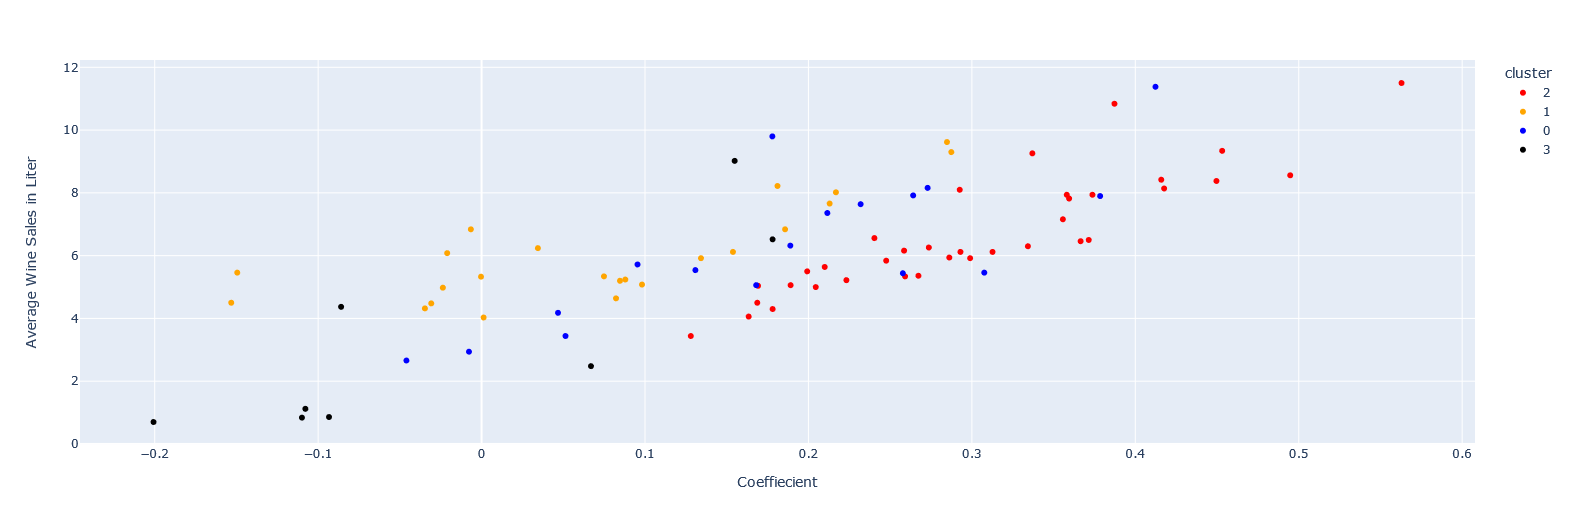
\includegraphics[scale = .29]{Graphs/Coeffiecient_scatter.png}
    \caption{Dendrogram}
    \label{fig:dendrogram}
\end{figure}

\begin{figure}[!htb]
    \centering
    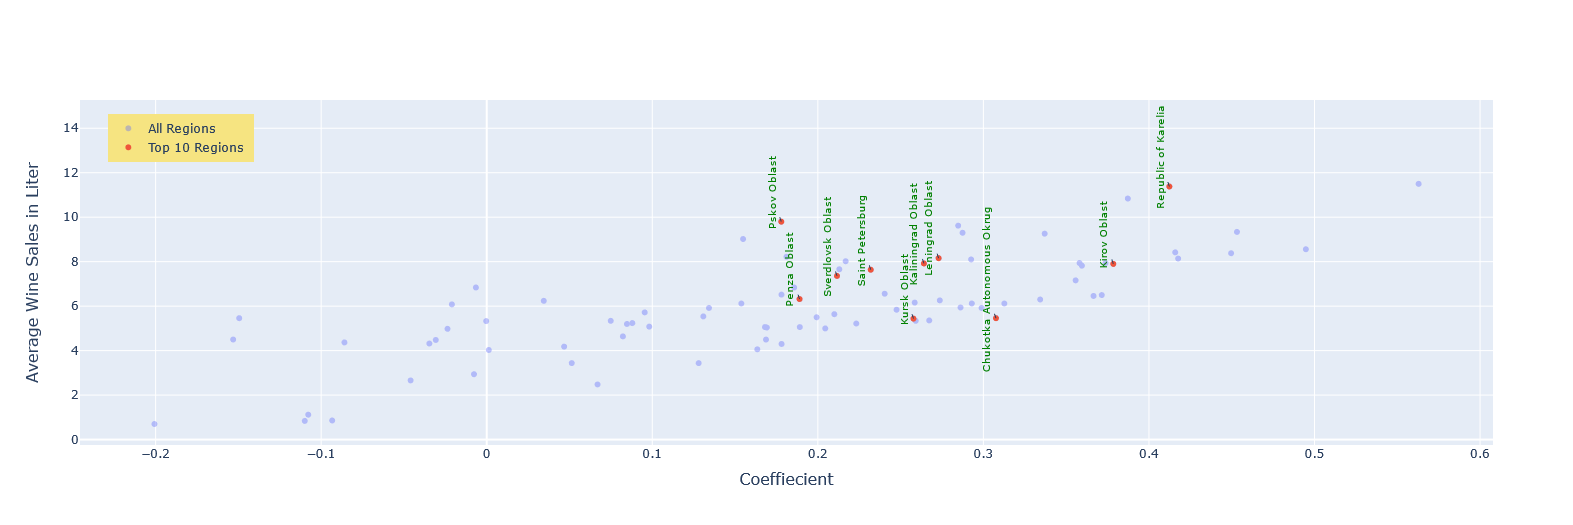
\includegraphics[scale = .3]{Graphs/Coefficent_scatter_target.png}
    \caption{Dendrogram}
    \label{fig:dendrogram}
\end{figure}



\end{document}

